\chapter{Travail}
\minitoc

%Dans chaque section (pour chaque pattern) : 
%Un résumé de ce qu'est le pattern, à quel problème il répond.
%Puis un schéma d'architecture localisée sur ce pattern.
%Expliquer quelques diagrammes de séquence.
%Choix d'implémentation, avantages et inconvénients du pattern.
\section{Travail}
%travail_decorator
\subsection{Décorateur}
\begin{figure}[h]
\begin{center}
    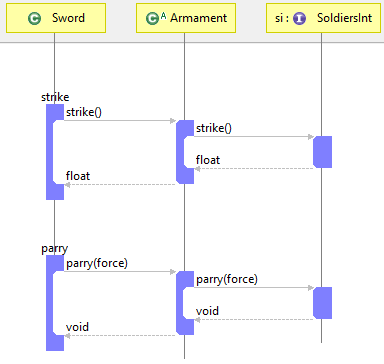
\includegraphics[width=11cm]{diagSeqDecorator}
\end{center}
    \caption{Diagramme de séquence du pattern décorateur}
    \label{sequence-decorateur}
\end{figure}
La première étape de conception du projet consistait à permettre à des soldats de disposer d'armements (un bouclier et une épée). Deux catégories de soldats devaient exister, les fantassins et les cavaliers, les soldats disposant d'un certain nombre de point de vie.

Pour réaliser cette première étape, nous avons commencé par créer les deux classes de soldats ainsi que deux classes d'armes. Afin d'anticiper le fait de pouvoir rajouter plus de catégories de soldat et plus d'armes, nous avons créé deux classes abstraites (Armament et SoldierAbstract).  

L'objectif était alors de pouvoir rajouter une ou plusieurs armes sur un soldat existant, et cela de façon dynamique, c'est à dire sans avoir à recréer le soldat. 

Pour répondre à cette problématique, nous avons utilisé le pattern Décorateur. 
Nous avons donc créé une classe SoldierInt représentant l'interface d'un soldat. Nous avons ensuite fait hériter notre classe SoldierAbstract de SoldierInt, et nous avons fait hérité notre classe Armament de SoldierInt, classe devenant notre décorateur puisque nous avons rajouté dans cette classe une référence à SoldierInt nous permettant ainsi de décorer notre soldat.

Ainsi donc, nous pouvons maintenant décorer un soldat avec des armes.

Une autre architecture possible aurait été de séparer les armes des soldats , ceci en créant un décorateur SoldierArmed avec comme sous classe SoldierWithShield et SoldierWithSword, ceci permettrait de séparer le comportement des armes du comportement des soldats, permettant ainsi de définir des méthodes spécifiques aux armes, sans en affecter les soldats, et vis vers ça. Cette solution a pour inconvénient de devoir rajouter plusieurs classes.

Une fois notre première architecture créé, nous avons rajouté la possibilité pour un soldat de porter des coups à ses adversaires (et à contrario de les parer) avec une vivacité dépendant de l'armement et de la catégorie du solat.

%travail_proxy
\subsection{Procurateur}
\begin{figure}[h]
\begin{center}
    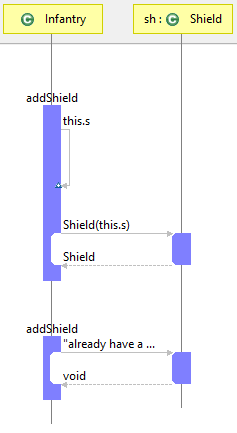
\includegraphics[width=11cm]{diagSeqProxy}
\end{center}
    \caption{Diagramme de séquence du pattern procurateur}
    \label{sequence-procurateur}
\end{figure}

Afin de contrôler les actions demandées par le client sur le soldat (comme par exemple l'ajout d'une nouvelle arme), nous avons appliqué le pattern Procuration nous permettant ainsi de fournir au client une représentation de l'objet soldat qui aura pour rôle ici de contrôler lors de l'ajout d'une arme sur un soldat si cette arme est déjà présente ou non sur le soldat.

Nous avons donc créé une interface Soldier contenant deux méthodes permettant d'ajouter des armes (addShield et addSword),interface héritant de notre classe SoldierInt. 
Les classes Infantry et Horsman ont quand à elle été dupliqués et implémentent l'interface Soldier (modifié par la suite car une classe abstraite implémente maintenant l'interface soldat afin d'éviter la duplication de code).

Enfin, nous avons rajouté une durée de vie à nos armes avec la variable RESISTANCE que nous avons placé dans nos classes d'armes (Shield et Sword). La résistance de l'arme diminue de 1point à chaque utilisation (c'est à dire à chaque appel de strike() ou de parry() ).

%travail_composite
\subsection{Composite}
\begin{figure}[h]
\begin{center}
    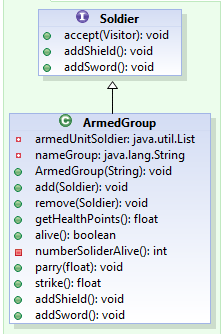
\includegraphics[width=11cm]{diagClassComposite}
\end{center}
    \caption{Diagramme de classes du pattern composite}
    \label{classes-composite}
\end{figure}

La seconde étape dans le projet consistait à rajouter la possibilité pour le client de créer des groupes armés. Un groupe armé de soldats peut être composé de plusieurs groupes armés, eux-mêmes décomposables en sous-groupes armés, et ainsi de suite. Cette notion de groupes armés fait ici apparaître une structure d'arbre avec des éléments composés d'autres éléments, structure qui fait penser à une hiérarchie. 
C'est pour cela que nous avons appliqué le pattern Composite, visible en figure \vref{classes-composite}, en créant une classe \emph{ArmedGroup} contenant une référence vers un objet \emph{Soldier} (qui représente notre \emph{procurateur}, ce que manipule le client).

Le seconde étape dans le projet consistait à rajouter la possibilité pour le client (et cela sans qu'il est besoin de s'en préoccuper) de créer des groupes armé, un groupe armé de soldats pouvant être composé de plusieurs groupes armés, eux-mêmes décomposés en sous-groupes armés, et ainsi de suite. Cette notion de groupe armé fait ici apparaître une structure d'arbre avec des éléments composé d'autres éléments, structure faisant apparaître une certaine hiérarchie. 
C'est donc pour cela que nous avons choisi de mettre en place le pattern Composite en créant une classe ArmedGroup contenant une référence de Soldier (qui est notre proxy, ce que manipule le client).

%travail_visitor
\subsection{Visiteur}
\begin{figure}[h]
\begin{center}
    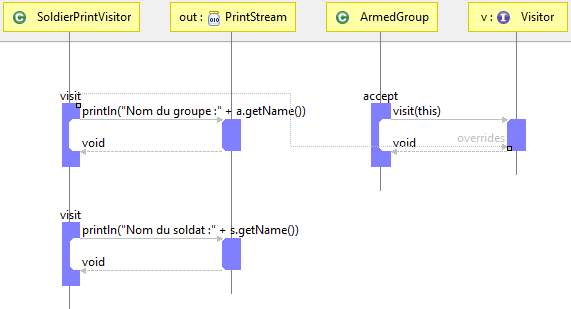
\includegraphics[width=11cm]{diagSeqVisitor}
\end{center}
    \caption{Diagramme de séquence du pattern visiteur}
    \label{sequence-visiteur}
\end{figure}

Nous avions à la fois des groupes armés ainsi que des soldats de différentes catégories. Afin de faciliter l'ajout de nouvelles fonctionnalités à la fois sur les groupes armés et sur les soldats, nous avons mis en place le pattern \emph{Visiteur}. Sans ce pattern, à chaque ajout de fonctionnalités, nous étions obligés de rajouter les méthodes dans nos classes \emph{Horseman}, \emph{Infantry} et \emph{ArmedGroup}, d'autant plus si nous voulions faire des traitement différents en fonction de chaque classe. Grâce au pattern \emph{Visiteur}, l'ajout de fonctionnalités supplémentaires (comme l'affichage de tous les soldats formant un groupe armé ou le comptage des effectifs de soldats par rapport à leur type au sein d’un groupe armé) se fait maintenant dans une seule classe, sans avoir à toucher le reste du code. Nous avons créé une classe \emph{SoldierPrintVisitor} pour ajouter la fonction d'affichage des soldats ainsi que la classe \emph{SoldierCountVisitor} pour ajouter la fonction de comptabilisation. Vous pouvez voir un exemple du déroulement des appels de méthodes en figure \vref{sequence-visiteur}. Tout ceci est totalement transparent vis-à-vis du reste du code : c'est là tout l'intérêt du pattern \emph{Visiteur}. On n'applique donc qu'un nombre minimal de modifications sur les autres classes de l'application et nous avons la possibilité de faire des traitements spécifiques pour chacune des classes de l'application. En résumé, nous pouvons maintenant ajouter des fonctionnalités sur les objets de notre choix sans toucher au reste du code.

Comme nous avions maintenant à la fois des groupes armé de soldats ainsi que des soldats de différente catégories, afin de faciliter l'ajout de nouvelles fonctionnalités à la fois sur les groupes armés et les soldats eux même, nous avons mis en place le pattern Visiteur. Sans ce pattern, à chaque ajout de fonctionnalité, nous étions obligé de rajouter les méthodes dans nos classes Horsman, Infantry et ArmedGroup, surtout si nous voulions faire des traitement différent en fonction de la classe. Grâce au pattern Visiteur, l'ajout de fonctionnalité supplémentaire (comme par exemple afficher tous les soldats formant un groupe armé ou encore compter des effectifs de soldats par rapport à leur type au sein d’un groupe armé) se fait maintenant dans une seule classe, sans avoir à toucher au reste du code. Nous avons donc par exemple créé une classe SoldierPrintVisitor pour ajouter la fonction d'affichage des soldats ainsi que la classe SoldierCountVisitor pour ajouter la fonction de comptabilisation, et tout ceci de manière totalement transparente vis à vis du reste du code, c'est là tout l’intérêt du pattern Visiteur, pas de modification à faire sur les autres classes de l'application et possibilité de faire des traitements spécifique pour chacune des classes de l'application. En résumé, nous pouvons maintenant ajouter des fonctionnalités sur les objets de notre choix sans toucher au reste du code.

%travail_observator
\subsection{Observateur}
\begin{figure}[h]
\begin{center}
    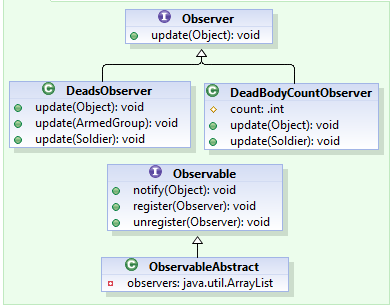
\includegraphics[width=11cm]{diagClassObserver}
\end{center}
    \caption{Diagramme de classes du pattern observeur}
    \label{classes-oberveur}
\end{figure}

Une des problématiques de ce projet était de pouvoir suivre le déroulement des conflits au fur et à mesure du déroulement de l’action. Nous aurions pu produire de nombreux print dans nos fonctions, ce qui aurait généré des affichages au fur et à mesure du déroulement des batailles. Cependant, cette méthode est peu flexible et peu maintenable ! 
C'est donc ici que le pattern \emph{Observateur} va être intéressant, car il nous permet d'observer un objet et d'être notifié de ses changements afin d'appliquer les traitements adéquats suite à ces changements. 
Ainsi, pour afficher au fur et à mesure les noms des soldats morts au sein d'un groupe armé ainsi que les armés détruites, nous avons mis en place le système visible en figure \vref{classes-oberveur}. Il est composé en premier lieu d'une interface \emph{Observer} avec pour sous-classe \emph{DeadsObserver}. Cette dernière se chargera de réaliser l'affichage. Nous avons également rendu observable notre classe \emph{ArmedGroup} en créant l'interface \emph{Observable}. \emph{ObservableAbstract} implémente cette interface et contient une liste d'\emph{Observers}, liste qui permet à l'objet, lorsqu'il change, d'en informer tous ses observateurs. 
Cette classe est également intéressante car elle permet de définir une interdépendance de type un à plusieurs, de tel façon que si on souhaite envoyer des télégrammes d’excuse à une liste d'ami une fois qu'un soldat meurt, on pourra notifier tous les objets qui dépendent du mort. L'inconvénient et la limite du pattern est que le graphe des relations d'observation peut vite devenir complexe. En effet, si l'on veut mettre en place le système des envois de télégrammes d’excuse à ses amis, c'est à dire à des soldats de l'armé, il va falloir que chaque objet soldat soit observé par tous les autres objets soldat « amis », ce qui implique la création de nombreux objet de type Observer (autant d'observer que de soldat) provoquant alors un ralentissement notable du programme ! Au vue de ces dernières remarques, nous n'avons pas retenu la fonction des télégramme via ce pattern là.

Une des autres problématiques de ce projet était de pouvoir suivre le déroulement des conflits au fur et à mesure de l’action. Une possibilité aurait été de faire de nombreux print dans nos fonctions, ce qui aurait produit des affichages au fur et à mesure du déroulement de la bataille, c'est à dire à chaque appel de parry() ou de strike(). Cependant, cette méthode n'est vraiment pas très pratique et pas du tout maintenable ! 
C'est donc ici que le pattern Observateur va être intéressant, en effet, il va nous permettre d'observer un objet et dès qu'il change, on va pouvoir être notifié de ce changement afin d'appliquer les traitements adéquat suite à ce changement d'état. 
Ainsi donc, pour afficher par exemple au fur et à mesure les noms des soldats morts au sein d'un groupe armé ainsi que les armés détruites, nous avons mit en place une interface Observer avec pour sous classe DeadsObserver, classe qui se chargera de réaliser l'affichage. Nous avons également rendu observable notre classe ArmedGroup en créant l'interface Observable. ObservableAbstract implémente cette interface et contient une liste d'Observer, une liste qui permettra donc à l'objet lorsqu'il change d'en informer tout ses observateurs. 
Cette classe est également intéressante ici car elle nous permet de définir une interdépendance de type un à plusieurs, de tel façon que si on souhaite envoyer des télégrammes d’excuse à une liste d'ami une fois qu'on est mort (même si cela n'est pas envisageable dans la vrai vie), grâce au pattern, on pourra notifier tout les objets qui dépende du mort (donc de l'objet qui est observé par sa liste d'amis). L'inconvénient et la limite ici du pattern est que le graphe peut vite devenir complexe. En effet, si l'on veut mettre en place le système des envoi de télégrammes d’excuse à ses amis, c'est à dire les soldats d'un même groupe par exemple, il va falloir que chaque objet soit observé par tout les autres objets « amis », ce qui va provoquer la création de plein d'objet de type Observable provoquant alors un ralentissement notable du programme ! Au vue de ces dernières remarques, nous n'avons pas retenu la fonction des télégramme via ce pattern là.

%travail_singleton
\subsection{Singleton}

Enfin, afin qu’il ne puisse y avoir qu'une seule instance de chaque observateur, nous avons mis en place le pattern Singleton, cela en donnant accès à l'instance de l'observateur via la méthode getInstance(), méthode qui renvoit la variable Instance  (déclaré en statique). Le constructeur est quand à lui rendu inaccessible.

%travail_abstract_factory
\subsection{Fabrique abstraite}
La dernière partie du projet consistait à créer plusieurs familles de soldats historiquement cohérentes, c'est à dire que pour une famille donnée, le type d'armement devait être conforme à son époque.

Pour le client, la notion d'époque vis à vis des armes doit rester transparente, en effet, on veut associer les bonnes armes au soldat construit par le client sans qu'il est à se soucier de la cohérence de son habillement, c'est à dire sans qu'il est à spécifier lui même les classes concrètes correspondant aux armes d'une époque ou d'une autre pour habiller son soldat. Ainsi donc, le client n'aura pas accès au processus de construction de son équipement (tel arme de défense pour telle époque, telle arme d'attaque pour telle époque), tout se fera automatiquement.

Pour réaliser cette demande, nous avons utilisé le pattern Fabrique abstraite. Nous avons donc créé une classe AbstractFactory comportant les méthodes setDefensiveWeapon(Soldier s) et setOffensiveWeapon(Soldier s) permettant d'affecter une arme défensive/offensive conforme à l'époque à un soldat donné. Ces méthodes se chargeront alors de la construction de l'équipement souhaité, en toute conformité avec l'époque. L'implémentation de ces deux méthodes se trouve dans les classes MiddleAgeFactory et ScienceFictionFactory, deux classes représentant deux époques différente. L'armement pourra donc être construit différemment en fonction de l'époque (par exemple les soldats de l'époque moderne seront équipés de laser).
Nous avons également rajouté des méthodes dans la fabrique permettant si besoin de construire des soldats de type différent.

Ainsi donc, grâce au pattern Fabrique abstraite nous pouvons garantir le maintient de la cohérence de nos équipements et de nos soldats en fonction de l'époque.
\section{Tests}

Afin de garantir la fiabilité de notre livrable, nous réalisons une série de tests unitaires et de tests fonctionnels. Les tests unitaires nous permettent de nous assurer du bon fonctionnement de certaines parties déterminées du logiciel. 

\subsection{Tests de la génération de combattants}
Nous réalisons un ensemble de génération de soldats tout en les équipant de pièces
d'armement puis nous vérifions la cohérence de leur force de frappe et de leur réaction
aux attaques adversaires.

\subsection{Tests de la génération de groupes armés}
Nous générons un ensembles de groupes composés de soldats puis nous vérifions que les groupes
sont bien cohérents par rapport aux combattants assignés.

\subsection{Tests des combats}
Nous faisons combattre des combattants et des groupes pour vérifier la cohérence de leurs réactions aux actions d'attaque et de défense.

\subsection{Tests des contraintes d'équipement}
Les combattants et groupes armés sont équipés d'une arme ou d'un bouclier puis ré-équipés d'un même type
d'armement pour vérifier qu'ils ne possèdent pas ensuite deux fois le même type d'équipement.

\subsection{Tests des observateurs}
Les observateurs doivent fournir un résultat prédéterminé pour des groupes armés ou des combattants sur
un scénario fixé. Nous vérifions que les résultats correspondent au scénario.

\subsection{Tests des fabriques}
Les fabriques doivent permettre de générer des combattants d'une époque particulière et d'équiper ces combattants
avec l'armement de l'époque. Nous testons que les combattants soient bien ceux attendus pour les époques du
moyen-age et du futur lointain. Nous testons également que leur équipement soit bien conforme à l'époque. Par
exemple, un \emph{Space marine} ne sera pas équipé d'une épée en bois, mais d'un laser.
